% Adjust these for the path of the theme and its graphics, relative to this file
%\usepackage{beamerthemeFalmouthGamesAcademy}
\usepackage{../../beamerthemeFalmouthGamesAcademy}
\usepackage{multimedia}
\graphicspath{ {../../} }

% Default language for code listings
\lstset{language=C++,
        morekeywords={each,in,nullptr}
}

% From http://blog.virtualglobebook.com/2011/02/syntax-highlighting-c-and-glsl-source.html

\lstdefinelanguage{GLSL}
{
sensitive=true,
morekeywords=[1]{
attribute, const, uniform, varying,
layout, centroid, flat, smooth,
noperspective, break, continue, do,
for, while, switch, case, default, if,
else, in, out, inout, float, int, void,
bool, true, false, invariant, discard,
return, mat2, mat3, mat4, mat2x2, mat2x3,
mat2x4, mat3x2, mat3x3, mat3x4, mat4x2,
mat4x3, mat4x4, vec2, vec3, vec4, ivec2,
ivec3, ivec4, bvec2, bvec3, bvec4, uint,
uvec2, uvec3, uvec4, lowp, mediump, highp,
precision, sampler1D, sampler2D, sampler3D,
samplerCube, sampler1DShadow,
sampler2DShadow, samplerCubeShadow,
sampler1DArray, sampler2DArray,
sampler1DArrayShadow, sampler2DArrayShadow,
isampler1D, isampler2D, isampler3D,
isamplerCube, isampler1DArray,
isampler2DArray, usampler1D, usampler2D,
usampler3D, usamplerCube, usampler1DArray,
usampler2DArray, sampler2DRect,
sampler2DRectShadow, isampler2DRect,
usampler2DRect, samplerBuffer,
isamplerBuffer, usamplerBuffer, sampler2DMS,
isampler2DMS, usampler2DMS,
sampler2DMSArray, isampler2DMSArray,
usampler2DMSArray, struct},
morekeywords=[2]{
radians,degrees,sin,cos,tan,asin,acos,atan,
atan,sinh,cosh,tanh,asinh,acosh,atanh,pow,
exp,log,exp2,log2,sqrt,inversesqrt,abs,sign,
floor,trunc,round,roundEven,ceil,fract,mod,modf,
min,max,clamp,mix,step,smoothstep,isnan,isinf,
floatBitsToInt,floatBitsToUint,intBitsToFloat,
uintBitsToFloat,length,distance,dot,cross,
normalize,faceforward,reflect,refract,
matrixCompMult,outerProduct,transpose,
determinant,inverse,lessThan,lessThanEqual,
greaterThan,greaterThanEqual,equal,notEqual,
any,all,not,textureSize,texture,textureProj,
textureLod,textureOffset,texelFetch,
texelFetchOffset,textureProjOffset,
textureLodOffset,textureProjLod,
textureProjLodOffset,textureGrad,
textureGradOffset,textureProjGrad,
textureProjGradOffset,texture1D,texture1DProj,
texture1DProjLod,texture2D,texture2DProj,
texture2DLod,texture2DProjLod,texture3D,
texture3DProj,texture3DLod,texture3DProjLod,
textureCube,textureCubeLod,shadow1D,shadow2D,
shadow1DProj,shadow2DProj,shadow1DLod,
shadow2DLod,shadow1DProjLod,shadow2DProjLod,
dFdx,dFdy,fwidth,noise1,noise2,noise3,noise4,
EmitVertex,EndPrimitive},
morekeywords=[3]{
gl_VertexID,gl_InstanceID,gl_Position,
gl_PointSize,gl_ClipDistance,gl_PerVertex,
gl_Layer,gl_ClipVertex,gl_FragCoord,
gl_FrontFacing,gl_ClipDistance,gl_FragColor,
gl_FragData,gl_MaxDrawBuffers,gl_FragDepth,
gl_PointCoord,gl_PrimitiveID,
gl_MaxVertexAttribs,gl_MaxVertexUniformComponents,
gl_MaxVaryingFloats,gl_MaxVaryingComponents,
gl_MaxVertexOutputComponents,
gl_MaxGeometryInputComponents,
gl_MaxGeometryOutputComponents,
gl_MaxFragmentInputComponents,
gl_MaxVertexTextureImageUnits,
gl_MaxCombinedTextureImageUnits,
gl_MaxTextureImageUnits,
gl_MaxFragmentUniformComponents,
gl_MaxDrawBuffers,gl_MaxClipDistances,
gl_MaxGeometryTextureImageUnits,
gl_MaxGeometryOutputVertices,
gl_MaxGeometryOutputVertices,
gl_MaxGeometryTotalOutputComponents,
gl_MaxGeometryUniformComponents,
gl_MaxGeometryVaryingComponents,gl_DepthRange},
morecomment=[l]{//},
morecomment=[s]{/*}{*/},
morecomment=[l][keywordstyle4]{\#},
}


% For strikethrough effect
\usepackage[normalem]{ulem}
\usepackage{wasysym}

\usepackage{pdfpages}

\usepackage{caption}
\captionsetup[figure]{font=scriptsize,labelfont=scriptsize}

% http://www.texample.net/tikz/examples/state-machine/
\usetikzlibrary{arrows,automata}

\newcommand{\modulecode}{COMP260}\newcommand{\moduletitle}{Distributed Systems}\newcommand{\sessionnumber}{5}

\begin{document}
\title{\sessionnumber: Debugging \& Optimisation for Graphics}
\subtitle{\modulecode: \moduletitle}

\frame{\titlepage} 

\begin{frame}{Learning outcomes}
	By the end of this week, you should be able to:
	\begin{itemize}
		\item \textbf{Recall} alternative ways to represent mesh vertices in memory.
		\item \textbf{Apply} basic transforms using the GLM library.
		\item \textbf{Explain} the constituents of the model-view-projection matrix and how it can be used to create a first-person camera controller.
	\end{itemize}
\end{frame}

\begin{frame}{Agenda}
	\begin{itemize}
		\pause\item Lecture (async):
		\begin{itemize}
			\item \textbf{Compare} different ways to store vertex data in memory.
			\item \textbf{Review} the transforms required to display 3D objects on a 2D screen.
		\end{itemize}
		\pause\item Workshop (sync):
		\begin{itemize}
			\item \textbf{Adapt} our basic triangle implementation to draw meshes with multiple triangles efficiently.
			\item \textbf{Experiment} with creating transforms using GLM and using them to move objects and the camera.
		\end{itemize}
	\end{itemize}
\end{frame}

\part{Writing Good Code}
\frame{\partpage}

\begin{frame}{Programming Aims}
	\begin{enumerate}
		\item\pause Make it work
		\item\pause Make it not break - \textbf{debugging}
		\item\pause Make it work quickly - \textbf{profiling \& optimisation}
		\item\pause Make it readable and maintainable - \textbf{code design}
	\end{enumerate}
\end{frame}

\begin{frame}{Other People's Code}
	\begin{center}
		\begin{figure}[h!]
			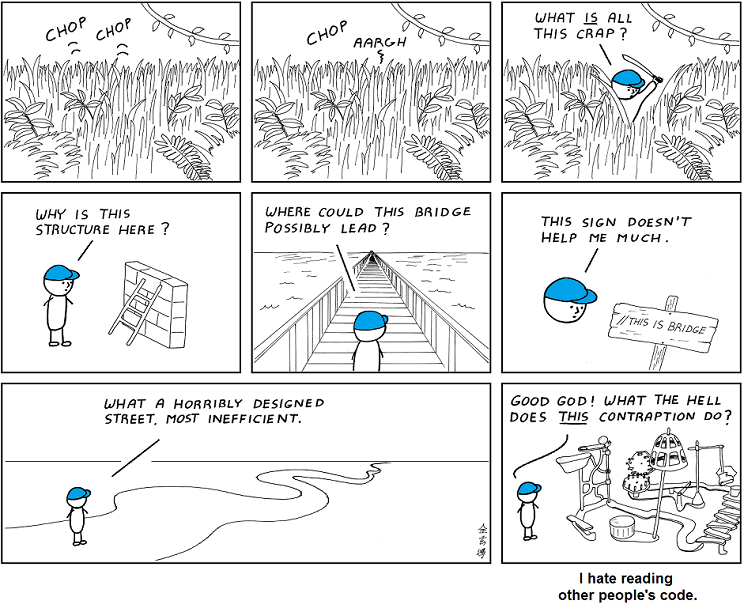
\includegraphics[height=0.8\textheight]{opc}
			\caption*{Image source: \url{https://abstrusegoose.com/432}}
		\end{figure}
	\end{center}
\end{frame}
\part{Debugging}
\frame{\partpage}

\begin{frame}{OpenGL Error States}
	\begin{itemize}
		\pause\item \lstinline{glGetError()} queries behind-the-scenes error flags to check state.
		\pause\item Possible \lstinline{glEnum} error codes for each function are listed in the documentation, e.g. for glBindTexture:
	\end{itemize}
	\begin{figure}[h!]
		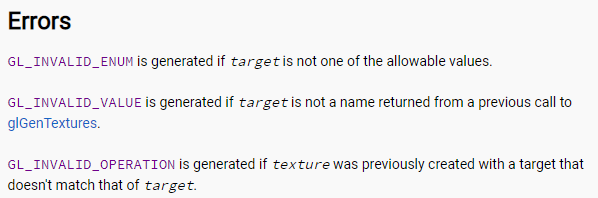
\includegraphics[width=0.8\textwidth]{glerrors}
	\end{figure}
\end{frame}

\begin{frame}[fragile]{Debug Output}
	\begin{itemize}
		\pause\item Extension made core feature from v4.3
		\pause\item Includes information about the cause and severity.
	\end{itemize}
	\pause\begin{lstlisting}
SDL_GL_SetAttribute(SDL_GL_CONTEXT_FLAGS,
		SDL_GL_CONTEXT_DEBUG_FLAG);	// Set up debug context
glEnable(GL_DEBUG_OUTPUT);
glEnable(GL_DEBUG_OUTPUT_SYNCHRONOUS);
glDebugMessageCallback(debugMessage, NULL);
glDebugMessageControl(GL_DONT_CARE, GL_DONT_CARE,
		GL_DONT_CARE, 0, NULL, GL_TRUE);	// Filter errors

// Callback
void APIENTRY debugMessage(GLenum source, GLenum type,
	GLuint id, GLenum severity, GLsizei length,
	const GLchar *message, const void *userParam) {
	// Do something with the error info
	// (print, write to file etc.)
}
	\end{lstlisting}
\end{frame}

\begin{frame}{Debugging Shaders}
	\begin{itemize}
		\pause\item Basic information from \textbf{compilation error reports}.
		\pause\item OpenGL GLSL \textbf{reference compiler} tests shader code against OpenGL specification.
		\pause\item Can use \textbf{colour channels} to display values.
		\pause\item Display \textbf{framebuffer contents} in the corner of the screen (similar to post-processing setup).
		\pause\item More detailed inspection requires using a \textbf{3rd party tool} (depending on GPU vendor etc.).
	\end{itemize}
\end{frame}
\part{Profiling \& Optimisation}
\frame{\partpage}

\begin{frame}{Writing Efficient GPU Code}
	\begin{itemize}
		\pause\item Same key principles apply as for CPU code!
		\pause\item Certain operations are optimised in GLSL, eg. swizzling, built-in functions for linear interpolation, dot product etc.
		\pause\item Write as much as possible in the vertex shader - remember there are fewer vertices than pixels!
		\pause\item As always: base your changes on profiling results...
	\end{itemize}
\end{frame}

\begin{frame}{Next steps}
	\begin{itemize}
		\item \textbf{Review} the additional asynchronous material for more information and resources on code design, debugging and profiling.
	\end{itemize}
\end{frame}

\end{document}

